% Ubah judul dan label berikut sesuai dengan yang diinginkan.
\section{Metode Penelitian}
\label{sec:MetodePenelitian}

Penelitian ini dilaksanakan sesuai sistem berikut dengan implementasinya. Desain sisttem merupakan konsep dari pembuatan dan perancangan infrastruktur yang kemudian diwujudkan dallam bentuk blok diagram alur ang harus dikerjakan. Pada Gambar \ref{fig:BlokMetodologi} menunjukkan bagan umum metodologi sistem.

\begin{figure} [ht]
  \centering
  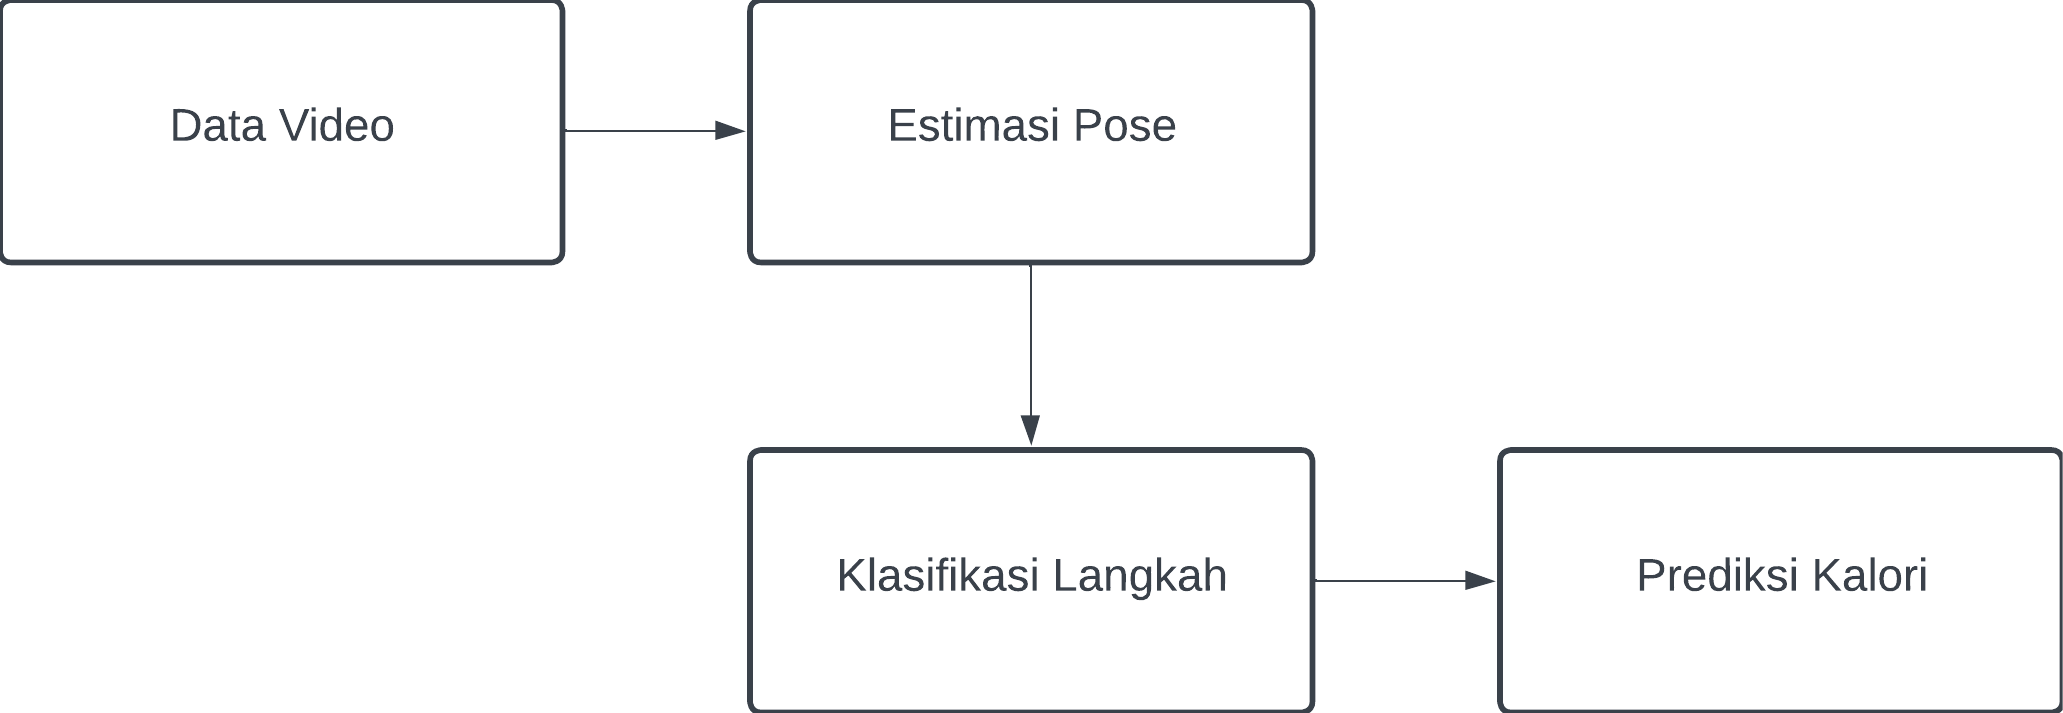
\includegraphics[width=0.4\textwidth]{gambar/blok diagram metodologi4.png}
  \caption{Bagan Umum Metodologi Sistem}
  \label{fig:BlokMetodologi}
\end{figure}

\subsection{Pengambilan Data}
\label{subsec:PengambilanData}

Pada tahap pertama yaitu pengambilan data, data diperoleh menggunakan kamera Webcam yang dimiliki oleh laptop atau kamera Webcam eksternal yang dihubungkan pada laptop ataupun komputer. Proses pengambilan data dilakukan dengan peraga melakukan aktivitas pada treadmill dengan ditampakkan secara jelas pada tampilan kamera Webcam. Setelah terdapat peraga dan tampak jelas pada tampilan maka data citra akan dilakukan pada tahap selanjutnya untuk dideteksi dan segmentasi pose seperti pada Gambar \ref{fig:PengambilanData}.

\begin{figure} [ht]
  \centering
  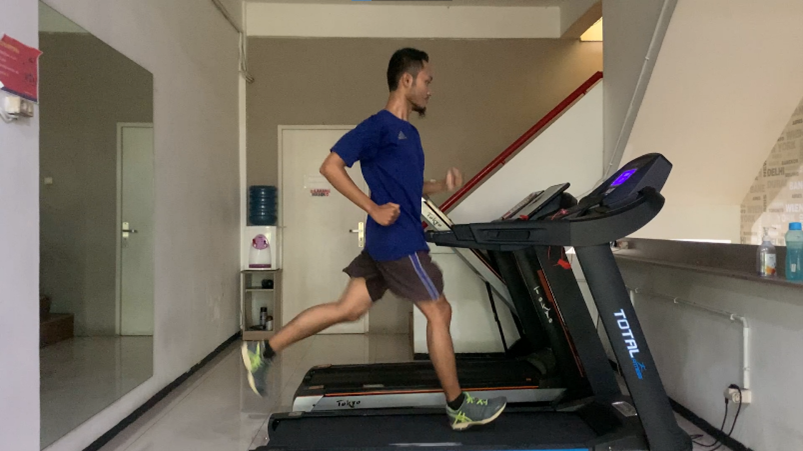
\includegraphics[width=0.4\textwidth]{gambar/pengambilan data.png}
  \caption{Proses Pengambilan Data}
  \label{fig:PengambilanData}
\end{figure}

\subsection{Deteksi Pose}
\label{subsec:DeteksiPose}

Deteksi dari hasil citra untuk dapat mengetahui bentuk postur tubuh manusia menggunakan Python dengan library OpenCV yaitu MediaPipe. Metode yang digunakan pada MediaPipe menggunakan deteksi pose untuk mendeteksi postur tubuh. Segementasi dilakukan dengan cara peraga melakukan aktivitas jogging pada treadmill dengan menentukan pose melangkah seperti yang terdapat pada Gambar \ref{fig:DeteksiPose}.

\begin{figure} [ht]
  \centering
  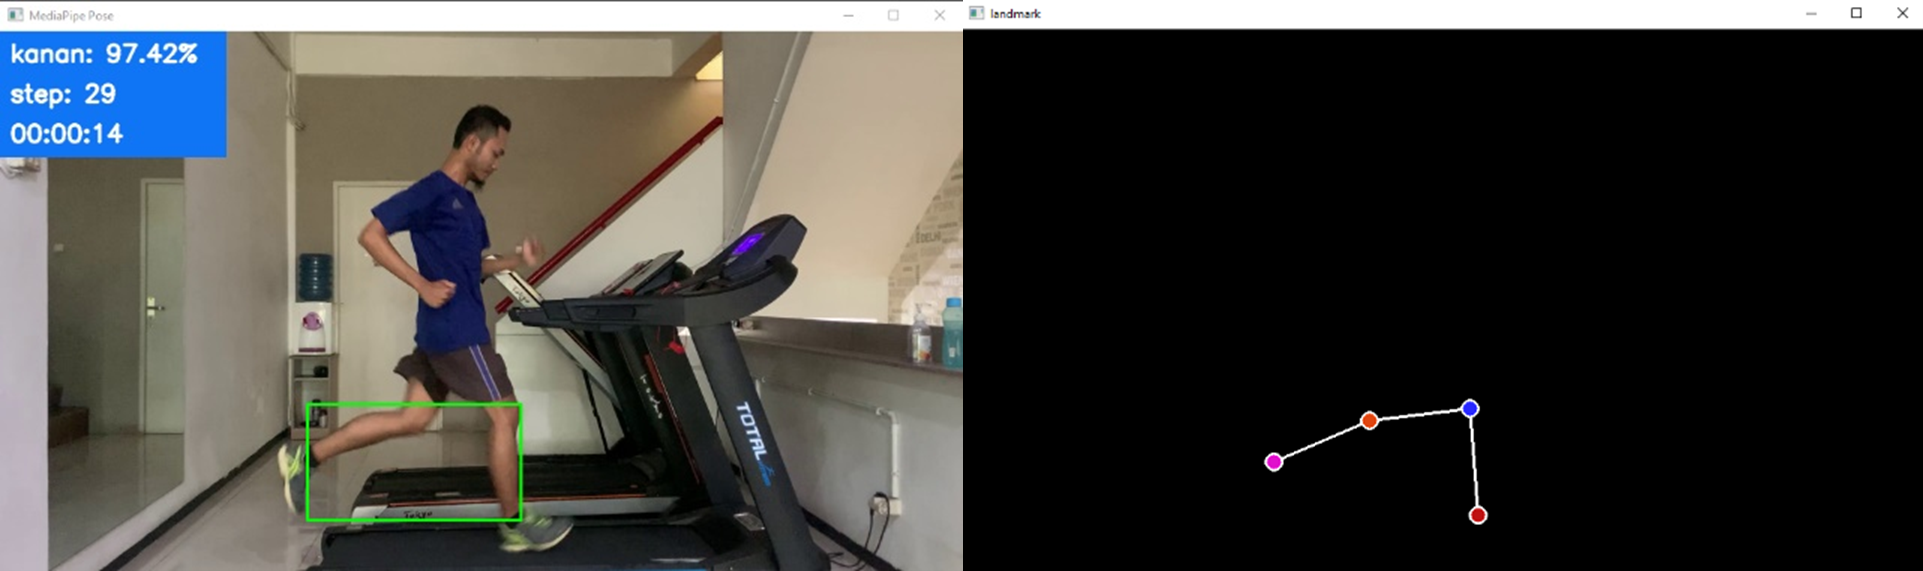
\includegraphics[width=0.4\textwidth]{gambar/deteksi pose.png}
  \caption{Deteksi Pose dengan Mediapipe}
  \label{fig:DeteksiPose}
\end{figure}

Fitur dibuat berdasarkan segmentasi pose yang telah ditentukan dan dilakukan deteksi. Semua fitur dipersiapkan sebagai kombinasi dataset yang nantinya akan digunakan pada training. Setelah menentukan fitur yang akan diekstrak, dilakukan ekstrak fitur untuk mendapatkan setiap data yang dibutuhkan dengan setiap percobaan dari kombinasi segmentasi pose. Hasil yang didapat dari ekstrak fitur berupa data set yang nantinya akan dilakukan training untuk model yang diinginkan. Dataset yang digunakan terdiri dari dua kelas dan pelabelan dari hasil deteksi dan estimasi pose, yaitu kaki “kiri” dan “kanan” seperti pada Gambar \ref{fig:DeteksiPose2}.

\begin{figure} [ht]
  \centering
  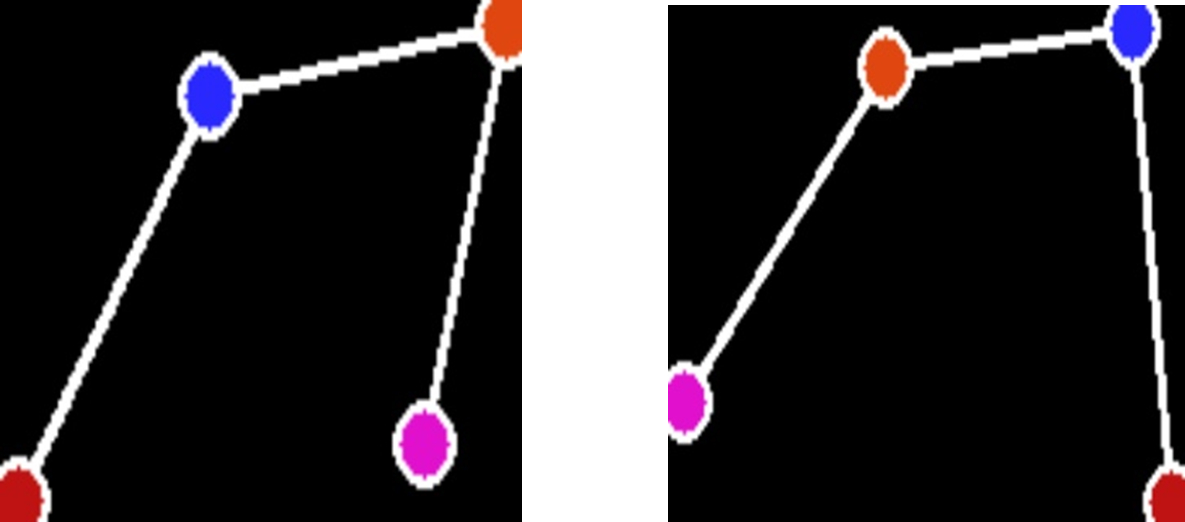
\includegraphics[width=0.4\textwidth]{gambar/deteksi pose2.png}
  \caption{Dataset Pembuatan Model}
  \label{fig:DeteksiPose2}
\end{figure}

\subsection{Model}
\label{subsec:Model}

Fitur yang telah dilakukan ekstraksi maka kemudian dilakukan training untuk memperoleh model deteksi. Model deteksi dari data set akan digunakan untuk melatih model dari sebuah algoritma pada Machine Learning. Dalam melakukan klasifikasi menggunakan Convolutional Neural Networks (CNN). Proses training ini bertujuan agar nantinya komputasi yang dilakukan dalam proses deteksi akan dapat diolah berdasarkan akuisisi data citra menjadi bentuk atau pola pemahaman yang diinginkan. Hasil training akan didapatkan model yang digunakan untuk melakukan klasifikasi atas dataset yang dimiliki yaitu terdapat dua kelas atau label untuk dapat diklasifikasikan menjadi kaki “kiri” dan “kanan”. Klasifikasi dalam menentukan aktivitas yang digunakan pada penelitian ini adalah dapat mengetahu langkah dari seseorang yang berjalan atau berlari seperti pada Gambar \ref{fig:DeteksiModel}.

\begin{figure} [ht]
  \centering
  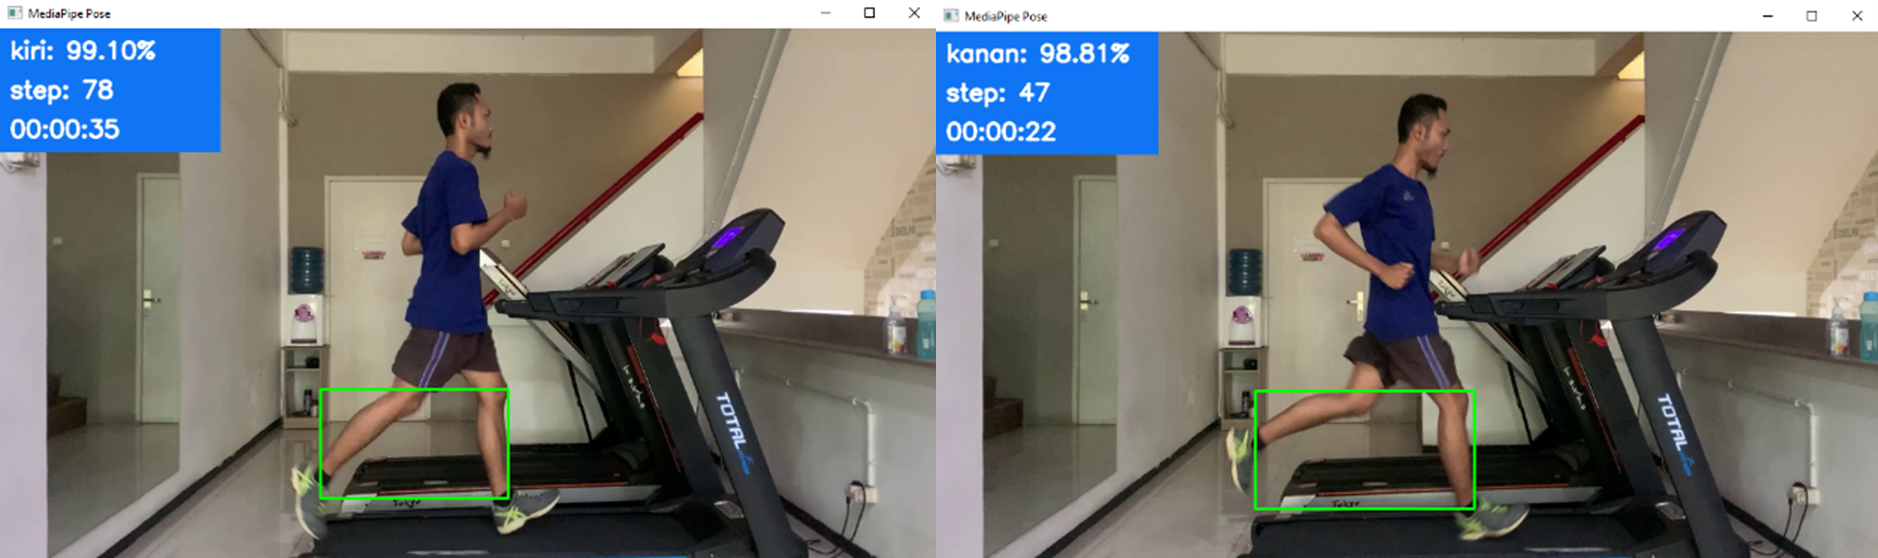
\includegraphics[width=0.4\textwidth]{gambar/deteksi.png}
  \caption{Klasifikasi pada Data Citra}
  \label{fig:DeteksiModel}
\end{figure}


Bentuk hasil klasifikasi yang dibuat adalah mendeteksi pose aktivitas dengan dapat menghitung langkah dan waktu yang ditempuh. Nilai langkah dan waktu yang ditempuh akan digunakan dalam perhitungan selanjutnya. Banyaknya jumlah langkah yang didapat saat hasil deteksi digunakan sebagai nilai variable pertama yang akan digunakan dalam penentuan perhitungan kalori. Langkah dideteksi dan dihitung seberapa banyak langkah yang dilakukan saat proses deteksi. Waktu tempuh saat proses deteksi merupakan nilai variabel kedua yang akan digunakan dalam penentuan perhitungan kalori. Waktu tempuh dimulai saat dideteksi pertama kali nilai langkah yang ditemukan hingga saat akhir langkah tidak ada penambahan kembali yang menandakan proses deteksi telah selesai. Hasil deteksi akan ditampilkan seiring dengan proses deteksi yang dilakukan pada data citra seperti pada Gambar \ref{fig:HasilDeteksi}.

\begin{figure} [ht]
  \centering
  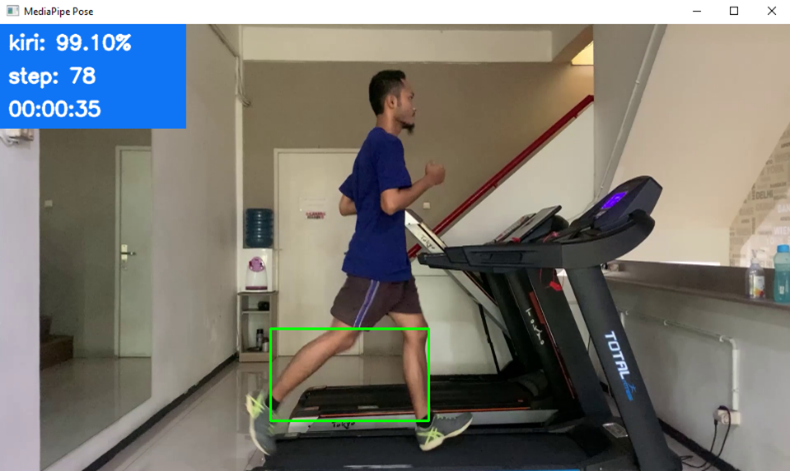
\includegraphics[width=0.4\textwidth]{gambar/hasil deteksi.png}
  \caption{Hasil Deteksi pada Citra}
  \label{fig:HasilDeteksi}
\end{figure}

\subsection{Prediksi Kalori}
\label{subsec:PrediksiKalori}

Prediksi kalori dilakukn dengan dua metode, yaitu menggunakan metode regresi linear dan menggunakan perhitungan rumus EC (Exercise Calories) berdasarkan satuan ukuran MET (Metabolic Equivalent). Kedua metode prediksi ini digunakan sebagai pembanding dalam melakukan analisa terhadap hasil yang didapatkan dari metode prediksi menggunakan metode regresi linear dengan perhitungan rumus. Data yang digunakanan dalam proses prediksi kalori diambil berdasarkan hasil klasifikasi dan hasil deteksi yang telah dilakukan sebelumnya. Hasil deteksi berupa banyaknya langkah dan waktu tempuh digunakan untuk proses prediksi kalori baik dengan metode regresi linear maupun metode perhitungan rumus.

\begin{enumerate}
  \item Regresi Linear
  
  Regresi merupakan suatu teknik analisis untuk mengidentifikasi relasi antar dua variabel atau lebih. Model regresi linear dilakukan dengan cara membuat dataset terlebih dahulu yang diatur sesuai dengan variabel-variabel yang dibutuhkan pada penelitian ini. Terdapat variabel independen dan variabel dependen sebagai bentuk model dataset yang akan digunakan pada regresi linear yang digunakan. Variabel independen yang digunakan pada dataset ini adalah waktu tempuh dan jarak tempuh. Sedangkan untuk variabel dependen yang digunakan adalah jumlah kalori yang terbakar.
  
  Dalam membuat model regresi linear, perlu dilakukan training dan pencarian dataset terlebih dahulu menggunakan alat bantu treadmill yang memiliki perhitungan jumlah kalori yang terbakar dengan menvariasikan sebanyak-banyaknya variabel yang akan digunakan pada model regresi linear. Setelah melakukan percobaan dan pencarian dataset maka akan didapatkan dataset untuk model regresi linear. Dengan didapatkannya model regresi linear, maka saat melakukan akuisisi data citra untuk diprediksi jumlah pembakaran kalori dengan menghasilkan hasil deteksi yang akan diregresikan dengan model regresi yang telah dimiliki dapat dilakukan prediksi jumlah pembakaaran kalori dari data citra tersebut.

  \item 
  
  Perhitungan Rumus 

  Perhitungan kalori dilakukan dengan mengacu pada nilai satuan ukuran MET (Metabolic Equivalent). Satuan MET akan mendapat pengukuran untuk konsumsi oksigen dan pembakaran kalori. Nilai dari satuan MET dapat didefinisikan pada Persamaan 1.

  \begin{equation}
    \label{eq:SatuanMET}
    1 \mathbf{MET} = 3,5 ml O_2  / KG / min
  \end{equation}

  Berdasarkan nilai satuan ukuran MET, didapatkan suatu persamaan untuk menghitung pembakaran kalori yang didefiniskan pada Persamaan 2.

  \begin{equation}
    \label{eq:RumusKalori}
    \mathbf{Cal} = \frac{MET  x 3.5 x BB}{200} x \frac{duration}{60} calories / min
  \end{equation}

  Pada persamaan pembakaran kalori yang akan digunakan untuk melakukan perhitungan pembakaran kalori dari aktivitas yang dilakukan dibutuhkan beberapa nilai variabel untuk mendapatkah hasil total pembakaran kalori, yaitu nilai MET, nilai berat badan (BB), dan nilai waktu tempuh dalam menit.

  Setiap aktivitas memiliki nilai MET yang berbeda-beda dan telah ditentukan oleh peneliti yang telah merangkum banyak aktivitas untuk ditentukan berapa nilai MET yang dihasilkan. Pada aktivitas olahraga yang difokuskan saat ini adalah jogging pada treadmill juga memiliki perbedaan nilai MET yang dipengaruhi oleh kecepatan jogging. Kecepatan aktivitas jogging dapat diketahui dengan nilai hasil deteksi berupa banyak langkah dan waktu tempuh untuk menentukan kecepatan dengan menggunakan Persamaan 3.

  \begin{equation}
    \label{eq:RumusKecepatan}
    \mathbf{Kecepatan} = \frac{Jarak}{Waktu}
  \end{equation}

  Untuk nilai jarak dilakukan dengan melakukan model regresi polinomial dari panjang langkah dari hasil kali kecepatan dan waktu yang dibagi dengan banyak langkah sesuai dataset yang diperoleh dari pengumpulan data pada treadmill. Model regresi digunakan untuk menentukan panjang jarak yang akan digunakan saat melakukan akuisisi data citra untuk dilakukan prediksi dengan menghasilkan data banyak langkah dan waktu tempuh. Kemudian banyak langkah akan dikalikan dengan hasil regresi untuk mentukan panjang langkah dan hasil pengalian tersebut dibagi dengan waktu tempuh untuk menemukan kecepatan. Dengan diperolehnya kecepatan maka dapat menentukan MET dengan membuat model regresi MET berdasarkan data yang telah dilakukan peneliti dan dapat dilanjutkan untuk mengetahui kalori dengan menggunakan rumus pada Persamaan 1.

\end{enumerate}

